\subsection{Essential matrix}
Two methods are implemented for essential matrix estimation: the $8$-point algorithm and the $5$ point algorithm~\cite{nister2003efficient}~\cite{li2006five}~\cite{triggs2000routines}~\cite{nister2004efficient}. $8$ point algorithm is chosen since it is the most straight-forward method which gives only one solution, while $5$ point algorithm is the minimal solution for essential matrix estimation. It is easy to derive from $5$ point algorithm to other $6$ or $7$ point algorithms, although the $6$ or $7$ point algorithms were proposed earlier than $5$ point algorithms.

The epipolar constraint on corresponding image points in two calibrated views can be written down as:
\begin{align}
\mathbf{q}'^T\mathbf{E}\mathbf{q}=0
\label{eq:c1}
\end{align}
where $\mathbf{E} \in \mathbb{R}^{3\times3}$ is the essential matrix. It is known that 
\begin{align}
\label{eq:c2}
det(\mathbf{E})=0 \\
\label{eq:c3}
\mathbf{E}^T\mathbf{EE}-\frac{1}{2}trace(\mathbf{E}^T\mathbf{E})\mathbf{E}=0
\end{align}
The usual way to compute essential matrix is to linearize relation~\eqref{eq:c1} into form $\mathbf{A}\mathbf{x} = 0$, where vector $\mathbf{x}$ contains nine elements of the matrix $\mathbf{E}$ and $\mathbf{A}$ contains image measurements. Essential matrix $\mathbf{E}$ is then constructed as a linear combination of the null space vectors of the matrix $\mathbf{A}$. The dimension of the null space depends on the number of point correspondences used. Additional constraints~\eqref{eq:c2} and~\eqref{eq:c3} are used to determine the coefficients
in the linear combination of the null space vectors or to project an approximate
solution to the space of correct essential matrices.

Generally speaking, methods differ with how they enforce~\eqref{eq:c2}~\eqref{eq:c3} constraints:
\begin{itemize}
	\item $8$ point method: since $\mathbf{E}$ is defined up to a scale $\lambda$, there are only $8$ independent unknowns and $1$ point pair constructs $1$ equation~\eqref{eq:c1}. As a result, $8$ point is enough to compute a result;
	\item $7$ point method: It is known that $\mathbf{E}$ is in the right null space of $\mathbf{A}$. With $7$ point, we can have $2$ null vectors $\mathbf{X},\ \mathbf{W}$, so $\mathbf{E}$ is a linear combination of the two null vectors. We define $\mathbf{E}=x\mathbf{X}+\mathbf{W}$ and then apply~\eqref{eq:c2} to form a $3^{rd}$ order polynomial over $x$. Solving for the real roots, we know $x$ and then $\mathbf{E}$.
	\item $5$ point method: $4$ null vectors $\mathbf{X},\ \mathbf{Y},\ \mathbf{Z},\ \mathbf{W}$ and $\mathbf{E}=x\mathbf{X}+y\mathbf{Y}+z\mathbf{Z}+\mathbf{W}$. By applying~\eqref{eq:c2} and~\eqref{eq:c3}, we will have ten multivariable polynomials. The solution follows by solve for $z$, then $x,\ y$ for obtaining $\mathbf{E}$. Up to $10$ reuslts may be returned.
\end{itemize}

\subsubsection{$5$ point algorithm}
\paragraph{Literature Review}
The 5-pt relative pose problem was studied already by Kruppa~\cite{Kruppa} who has shown that it has at most eleven solutions. Maybank and Faugeras~\cite then sharpened Kruppa’s result

The most widely known $5$ point algorithms or implementations are listed here:
\begin{enumerate}
\item Nist\'er version in CVPR~\cite{nister2003efficient} and PAMI~\cite{nister2004efficient}. The PAMI version is favoured here since it is relatively simpler.
\item Gr\"obner basis version in~\cite{stewenius2006recent}. 
\item Polynomial Eigenvalue solution in~\cite{kukelovapolynomial}.
\end{enumerate}
Implementations:
\begin{itemize}
\item \url{https://github.com/prateekt/allyourposesrours}: a \textsc{Matlab} symbolic based implementation of Nist\'er five point algorithm.
\item archived at \url{https://web.archive.org/web/20170401223934/http://www.vis.uky.edu:80/~stewe/FIVEPOINT/}: a \textsc{Matlab} based Grobner Basis Method and a Nist\'er five point implementation.
\item \url{https://raw.githubusercontent.com/jianxiongxiao/SFMedu/master/peig5pt.m}: Polynomial Eigenvalue solution.
\item: two self developed implementations.
\end{itemize}
Other implementation may be considered for benchmark if time is allowed\footnote{\url{https://github.com/SergioRAgostinho/five_point_algorithm}}.

A performance and runtime evaluation can be seen from
\begin{figure}
\centering
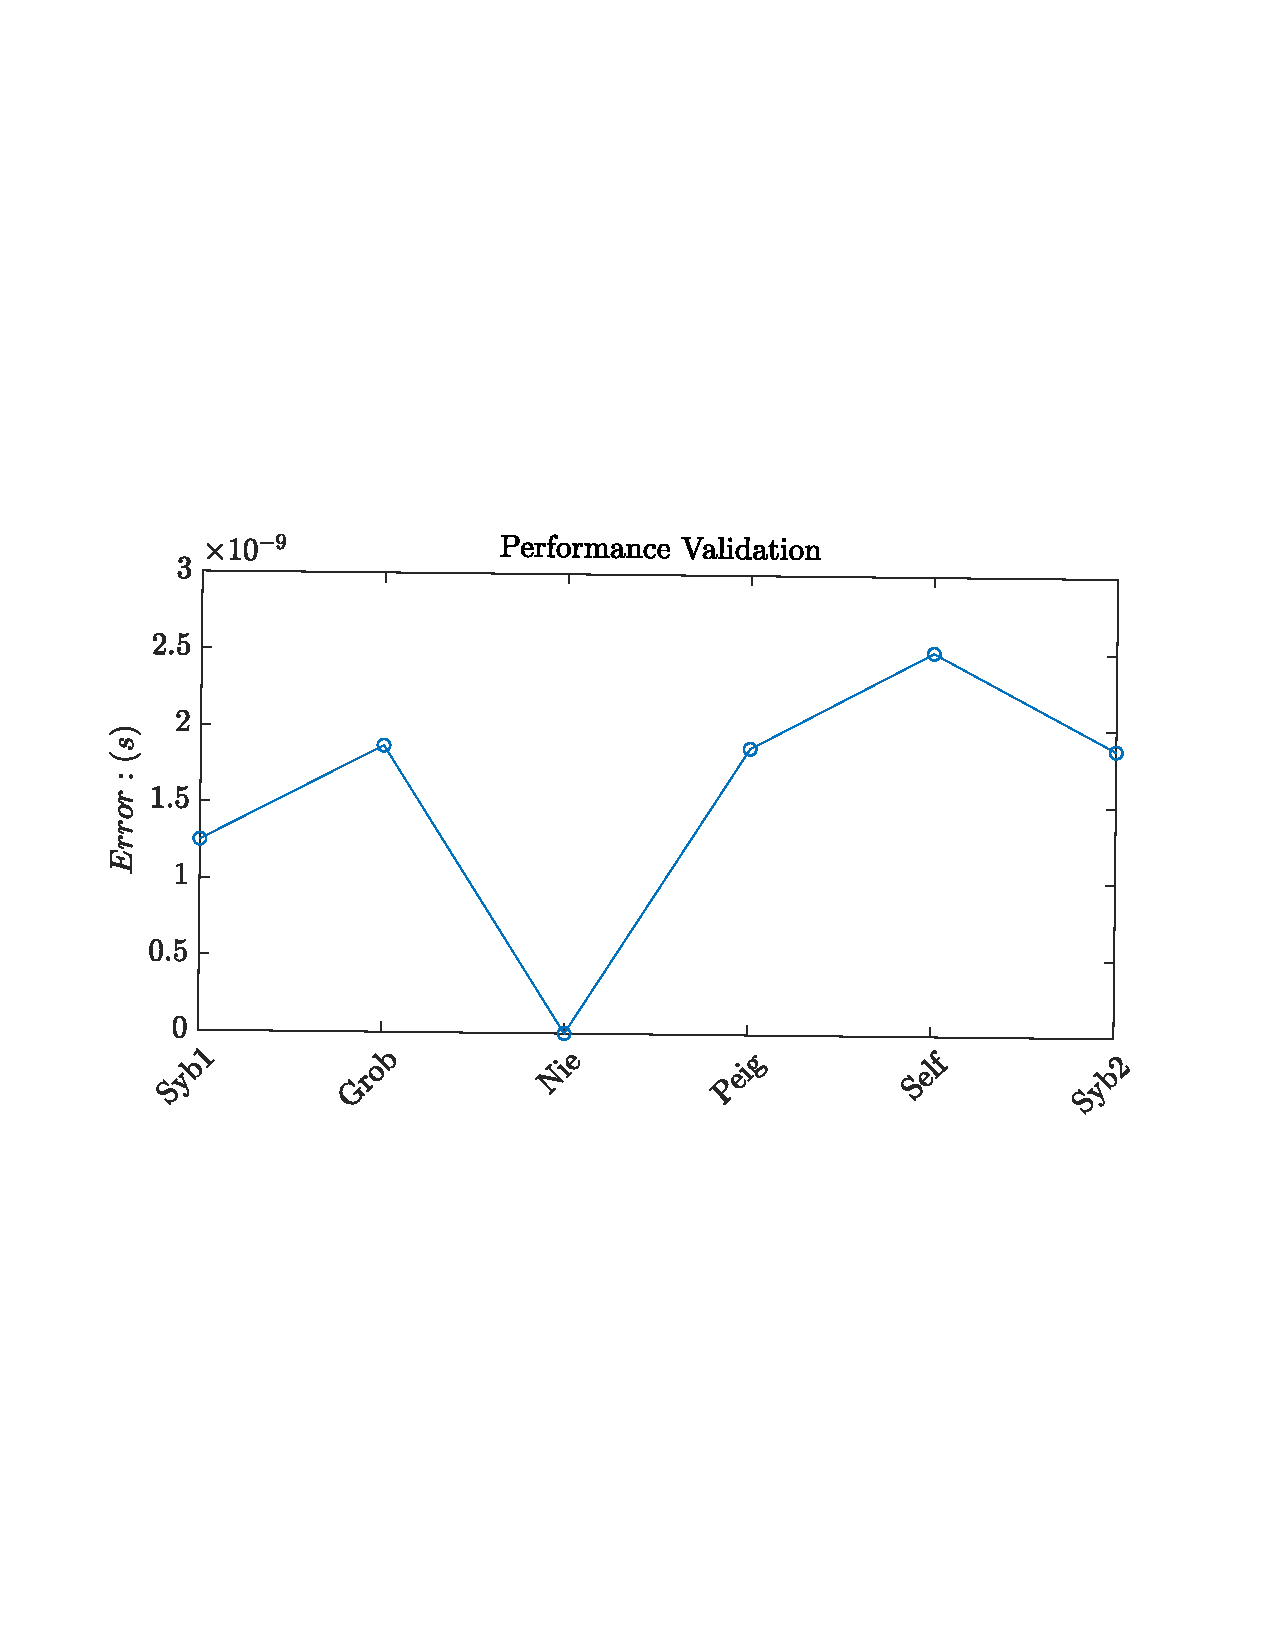
\includegraphics[width=0.45\textwidth]{hand_eye_files/vision/figures/five_point_perf}
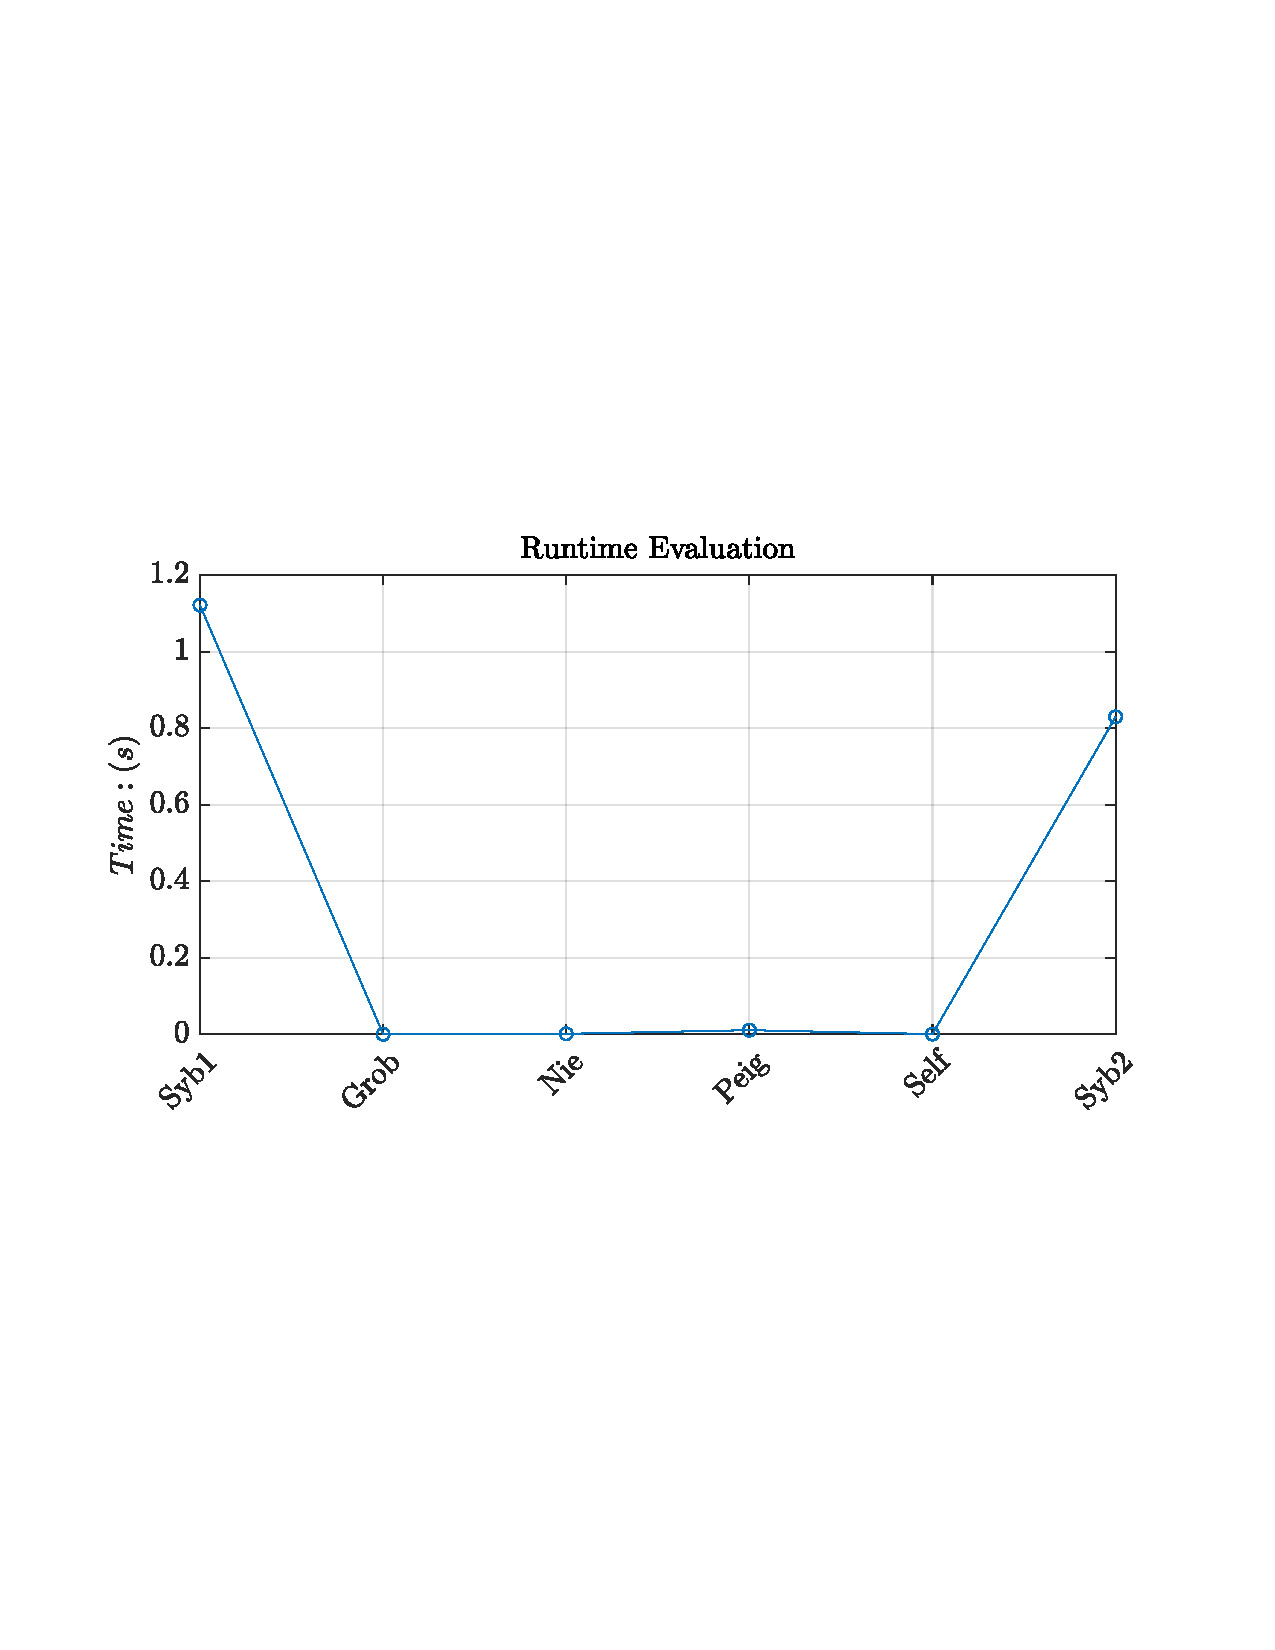
\includegraphics[width=0.45\textwidth]{hand_eye_files/vision/figures/five_point_time}
\label{fig:ess_com}
\end{figure}
\begin{table}[h!]
\centering
\caption{Details of runtime}
\begin{tabular}{c||c}
\hline
\textbf{Name} & \textbf{Time}: (s) \\
 Syb1 & $1.1213$ \\
 Grob & $0.0002$ \\
 Nie & $0.0015$ \\
 Peig & $0.0110$ \\
 Self & $0.0008$ \\
 Syb2 & $1.8294$ \\ 
 \hline
\end{tabular}
\label{tb:ess_com}
\end{table}
From this figure~\ref{fig:ess_com} and Table~\ref{tb:ess_com}, it can be seen Grob, Nie, Self are the three fastest methods. So they are chosen as the five point algorithm for future usage\footnote{$100$ Experiments are carried for evaluation.}.